\hypertarget{algorithmic-fairness}{%
\chapter{Algorithmic Fairness}\label{algorithmic-fairness}}

In the previous chapter, we replicated the analysis reported in
``Machine Bias'', by Julia Angwin, Jeff Larson, Surya Mattu and Lauren
Kirchner, published by ProPublica in May 2016.

After the ProPublica article, the Washington Post published a response
by Sam Corbett-Davies, Emma Pierson, Avi Feller and Sharad Goel: ``A
computer program used for bail and sentencing decisions was labeled
biased against Blacks. It's actually not that clear.''

I encourage you to read both of those articles before you go on. In this
chapter, I explain some of the arguments presented in the Washington
Post (WaPo) article, and we will replicate their analysis.

\hypertarget{the-response}{%
\section{The Response}\label{the-response}}

The Washington Post article summarizes the ProPublica article and the
response from Northpointe, the company that makes COMPAS, like this:

\begin{itemize}
\item
  ProPublica claims that COMPAS is unfair because ``among defendants who
  ultimately did not reoffend, Blacks were more than twice as likely as
  Whites to be classified as medium or high risk.''
\item
  Northpointe claims that COMPAS is fair because ``scores mean
  essentially the same thing regardless of the defendant's race. For
  example, among defendants who scored a seven on the COMPAS scale, 60
  percent of White defendants reoffended, which is nearly identical to
  the 61 percent of Black defendants who reoffended.''
\end{itemize}

So ProPublica and Northpointe are invoking different definitions of
``fair''.

In the previous chapter we explored the first definition by computing
error rates (false positive and false negative) for White and Black
defendants. In this chapter, we'll explore the second definition, which
is called ``calibration''.

\hypertarget{calibration}{%
\section{Calibration}\label{calibration}}

The WaPo article includes this figure, which shows ``White and Black
defendants with the same risk score are roughly equally likely to
reoffend.''

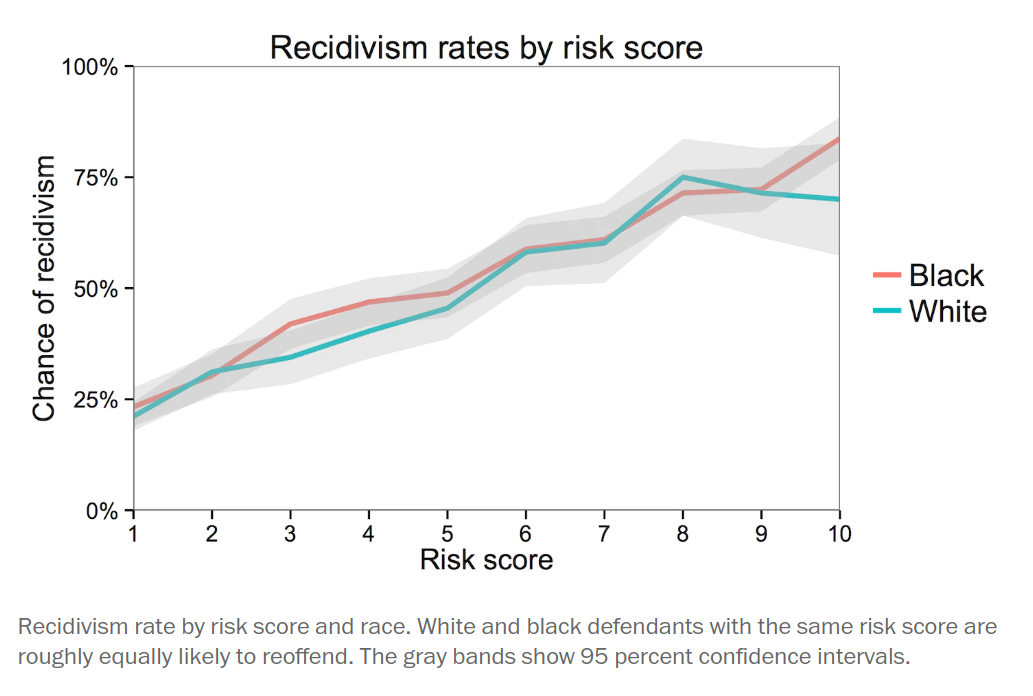
\includegraphics{chapters/figs/calibration1.png}

To understand this figure, let's start by replicating it.

The following function groups defendants by risk score and computes the
fraction in each group that were charged with another crime within two
years.

\begin{lstlisting}[]
def calibration_curve(df):
    """Fraction in each risk group charged with another crime.
    
    df: DataFrame
    
    returns: Series
    """
    grouped = df.groupby('decile_score')
    return grouped['two_year_recid'].mean()
\end{lstlisting}

The following figure shows this calibration curve for all defendants and
for White and Black defendants separately.

\begin{lstlisting}[]
cal_all = calibration_curve(cp)
cal_all.plot(linestyle='dotted', 
              color='gray',
              label='All defendants')

white = (cp['race'] == 'Caucasian')
cal_white = calibration_curve(cp[white])
cal_white.plot(label='White')

black = (cp['race'] == 'African-American')
cal_black = calibration_curve(cp[black])
cal_black.plot(label='Black')

decorate(xlabel='Risk score',
         ylabel='Fraction charged with new crime',
         title='Recivism vs risk score, grouped by race')
\end{lstlisting}

\begin{center}
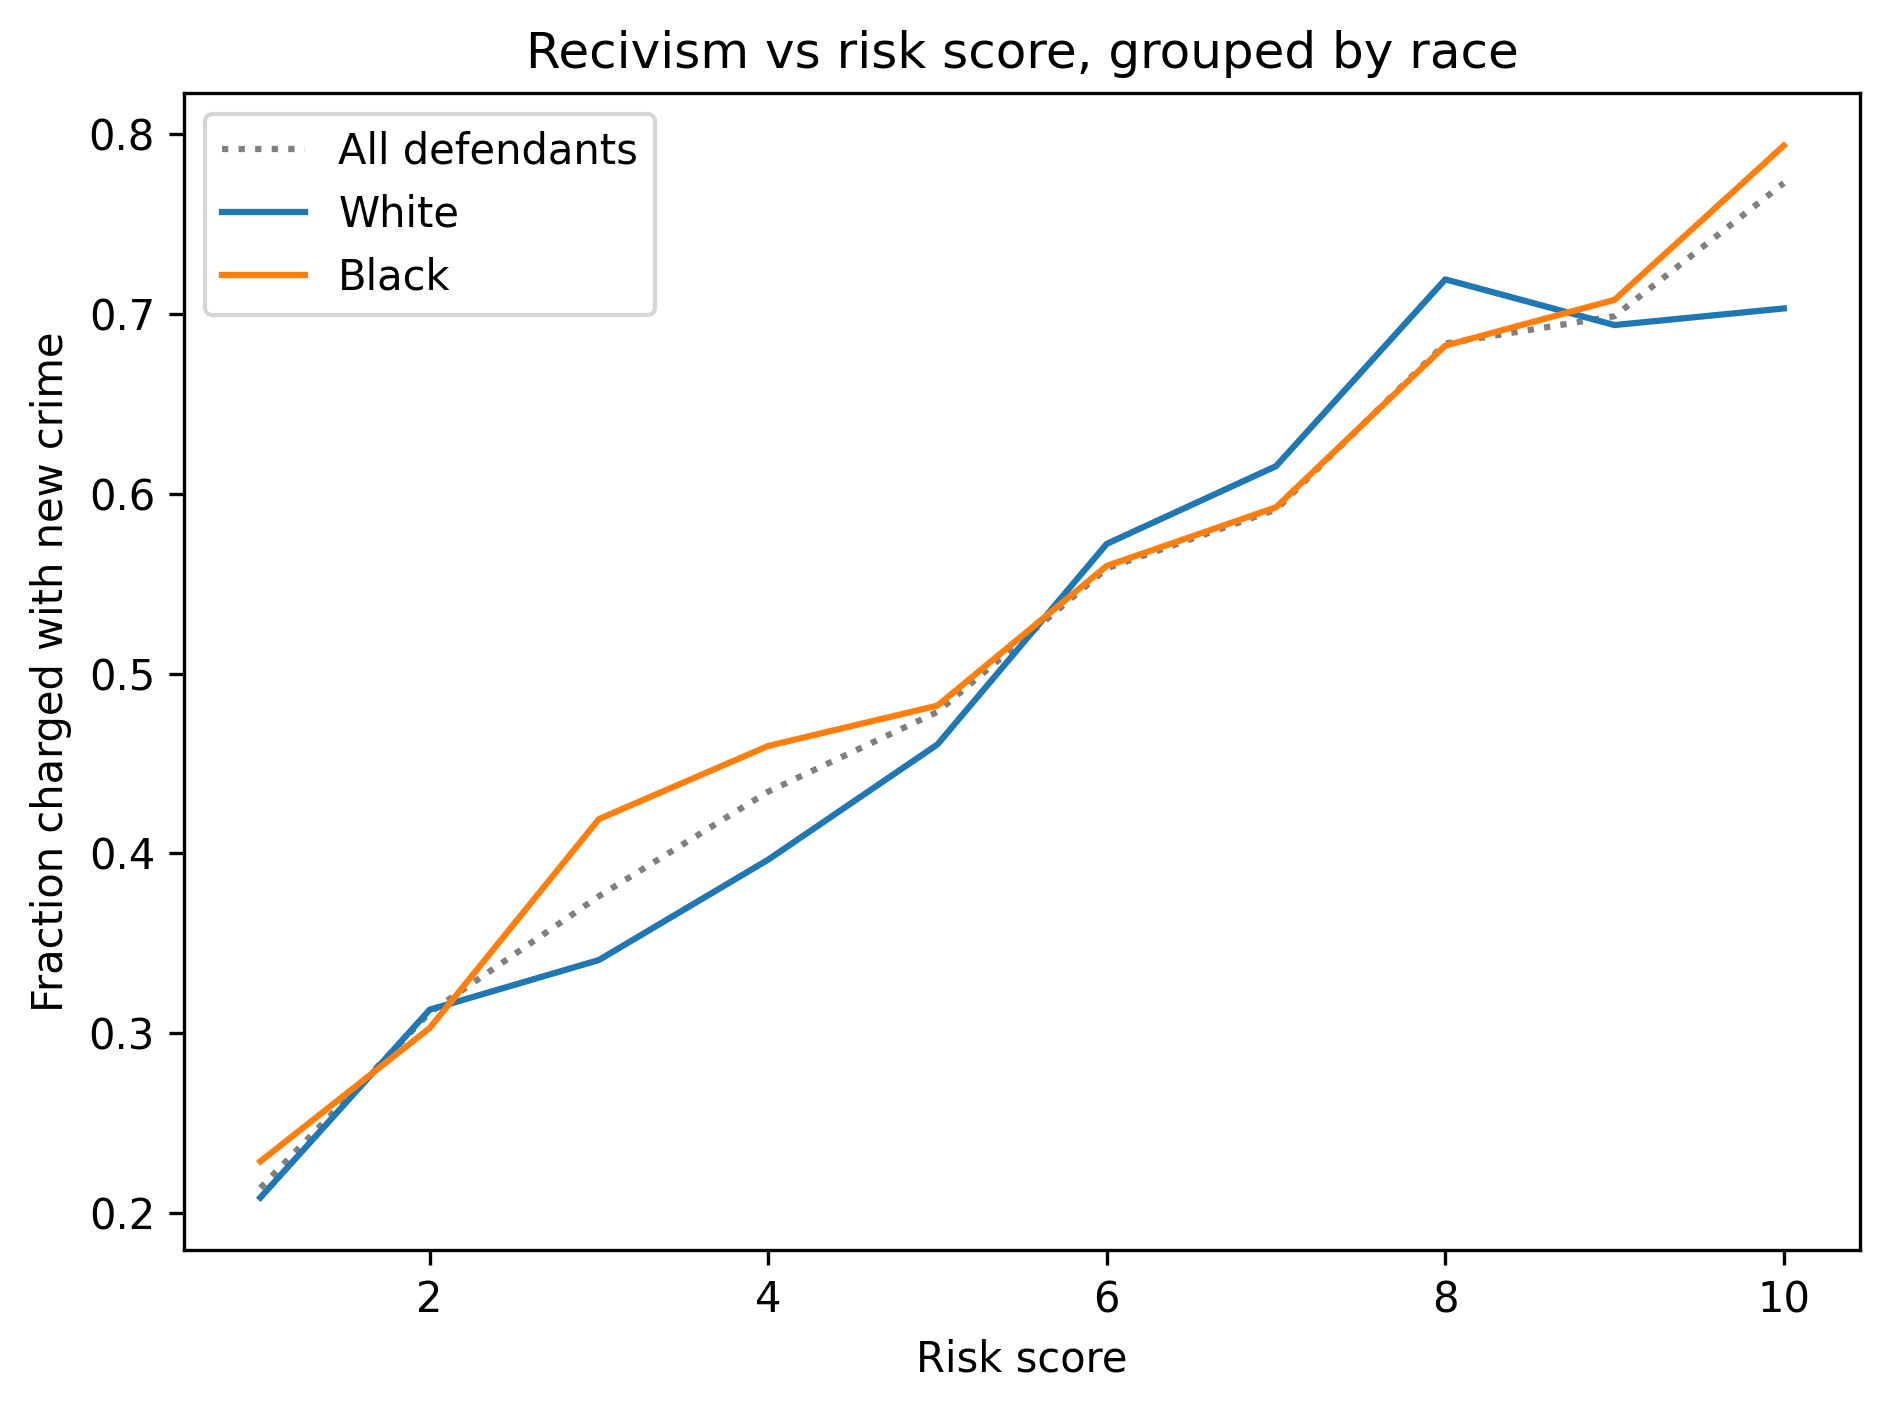
\includegraphics[width=4in]{chapters/02_calibration_files/02_calibration_20_0.png}
\end{center}

This figure shows that people with higher risk scores are more likely to
be charged with a new crime within two years. In that sense COMPAS works
as intended.

Furthermore, the test is equally \textbf{calibrated} for Black and White
defendants; that is, in each risk group, the rate of recidivism is about
the same for both groups.

The WaPo article explains why this is important:

\begin{quote}
A risk score of seven for Black defendants should mean the same thing as
a score of seven for White defendants. Imagine if that were not so, and
we systematically assigned Whites higher risk scores than equally risky
Black defendants with the goal of mitigating ProPublica's criticism. We
would consider that a violation of the fundamental tenet of equal
treatment.
\end{quote}

So we want a test that has the same calibration for all groups, and we
want a test that has the same error rates for all groups. But there's
the problem: it is mathematically impossible to be fair by both
definitions at the same time.

To see why, let's go back to the confusion matrix.

\hypertarget{matrices-and-metrics}{%
\section{Matrices and Metrics}\label{matrices-and-metrics}}

In the previous chapter, we computed confusion matrices for White and
Black defendants. Here they are again:

\begin{lstlisting}[]
matrix_white = make_matrix(cp[white])
matrix_white
(@\dashfill@)
@@@/home/downey/miniconda3/envs/ElementsOfDataScience/lib/python3.8/site-packages/IPython/core/formatters.py:342: FutureWarning: In future versions `DataFrame.to_latex` is expected to utilise the base implementation of `Styler.to_latex` for formatting and rendering. The arguments signature may therefore change. It is recommended instead to use `DataFrame.style.to_latex` which also contains additional functionality.
  return method()@@@
\end{lstlisting}

\begin{tabular}{lrr}
\midrule
Actual &  Condition &  No Condition \\
Predicted &            &               \\
\midrule
Positive  &        505 &           349 \\
Negative  &        461 &          1139 \\
\midrule
\end{tabular}

\begin{lstlisting}[]
matrix_black = make_matrix(cp[black])
matrix_black
(@\dashfill@)
@@@/home/downey/miniconda3/envs/ElementsOfDataScience/lib/python3.8/site-packages/IPython/core/formatters.py:342: FutureWarning: In future versions `DataFrame.to_latex` is expected to utilise the base implementation of `Styler.to_latex` for formatting and rendering. The arguments signature may therefore change. It is recommended instead to use `DataFrame.style.to_latex` which also contains additional functionality.
  return method()@@@
\end{lstlisting}

\begin{tabular}{lrr}
\midrule
Actual &  Condition &  No Condition \\
Predicted &            &               \\
\midrule
Positive  &       1369 &           805 \\
Negative  &        532 &           990 \\
\midrule
\end{tabular}

And here are the metrics we computed from the confusion matrices:

\begin{lstlisting}[]
metrics_white = compute_metrics(matrix_white, 
                                'White defendants')
metrics_white
(@\dashfill@)
@@@/home/downey/miniconda3/envs/ElementsOfDataScience/lib/python3.8/site-packages/IPython/core/formatters.py:342: FutureWarning: In future versions `DataFrame.to_latex` is expected to utilise the base implementation of `Styler.to_latex` for formatting and rendering. The arguments signature may therefore change. It is recommended instead to use `DataFrame.style.to_latex` which also contains additional functionality.
  return method()@@@
\end{lstlisting}

\begin{tabular}{lr}
\midrule
{} &    Percent \\
White defendants &            \\
\midrule
FPR              &  23.454301 \\
FNR              &  47.722567 \\
PPV              &  59.133489 \\
NPV              &  71.187500 \\
Prevalence       &  39.364303 \\
\midrule
\end{tabular}

\begin{lstlisting}[]
metrics_black = compute_metrics(matrix_black, 
                                'Black defendants')
metrics_black
(@\dashfill@)
@@@/home/downey/miniconda3/envs/ElementsOfDataScience/lib/python3.8/site-packages/IPython/core/formatters.py:342: FutureWarning: In future versions `DataFrame.to_latex` is expected to utilise the base implementation of `Styler.to_latex` for formatting and rendering. The arguments signature may therefore change. It is recommended instead to use `DataFrame.style.to_latex` which also contains additional functionality.
  return method()@@@
\end{lstlisting}

\begin{tabular}{lr}
\midrule
{} &    Percent \\
Black defendants &            \\
\midrule
FPR              &  44.846797 \\
FNR              &  27.985271 \\
PPV              &  62.971481 \\
NPV              &  65.045992 \\
Prevalence       &  51.433983 \\
\midrule
\end{tabular}

If we look at the error rates (FPR and FNR), it seems like COMPAS is
biased against Black defendants:

\begin{itemize}
\item
  Their false positive rate is higher (45\% vs 23\%): among people who
  \emph{will not} recidivate, Black defendants are more likely to be
  classified high risk.
\item
  Their false negative rate is lower (28\% vs 48\%): among people who
  \emph{will} recidivate, Black defendants are less likely to be
  classified low risk.
\end{itemize}

But if we look at the the predictive values (PPV and NPV) it seems like
COMPAS is biased in favor of Black defendants:

\begin{itemize}
\item
  Among people in the \emph{high risk group}, Black defendants are more
  likely to be charged with another crime (63\% vs 59\%).
\item
  Among people in the \emph{low risk group}, Black defendants are less
  likely to ``survive'' two years without another charge (65\% vs 71\%).
\end{itemize}

It seems like we should be able to fix these problems, but it turns out
that we can't. We'll see why in the next section.

\hypertarget{what-would-it-take}{%
\section{What Would It Take?}\label{what-would-it-take}}

Suppose we want to fix COMPAS so that predictive values are the same for
Black and White defendants. We could do that by using different
thresholds for the two groups. In this section, we'll figure out what it
would take to re-calibrate COMPAS; then we'll see what effect that would
have on predictive values.

The following function loops through possible thresholds, makes the
confusion matrix with each threshold, and computes accuracy metrics.

\begin{lstlisting}[]
def sweep_threshold(cp):
    """Sweep a range of threshold and compute accuracy metrics.
    
    cp: DataFrame of COMPAS data
    
    returns: DataFrame with one row for each threshold and
             one column for each metric
    """
    index = range(0, 11)
    columns = ['FPR', 'FNR', 'PPV', 'NPV', 'Prevalence']
    table = pd.DataFrame(index=index, columns=columns, dtype=float) 

    for threshold in index:
        m = make_matrix(cp, threshold)
        metrics = compute_metrics(m)
        table.loc[threshold] = metrics['Percent']
        
    return table
\end{lstlisting}

Here's the resulting table for all defendants.

\begin{lstlisting}[]
table_all = sweep_threshold(cp)
table_all.head()
(@\dashfill@)
@@@/home/downey/miniconda3/envs/ElementsOfDataScience/lib/python3.8/site-packages/IPython/core/formatters.py:342: FutureWarning: In future versions `DataFrame.to_latex` is expected to utilise the base implementation of `Styler.to_latex` for formatting and rendering. The arguments signature may therefore change. It is recommended instead to use `DataFrame.style.to_latex` which also contains additional functionality.
  return method()@@@
\end{lstlisting}

\begin{tabular}{lrrrrr}
\midrule
{} &         FPR &        FNR &        PPV &        NPV &  Prevalence \\
\midrule
0 &  100.000000 &   0.000000 &  45.065151 &        NaN &   45.065151 \\
1 &   71.435781 &   9.474008 &  50.969865 &  78.611111 &   45.065151 \\
2 &   55.084532 &  18.486620 &  54.831368 &  74.758505 &   45.065151 \\
3 &   43.325763 &  27.130114 &  57.978463 &  71.803069 &   45.065151 \\
4 &   32.349230 &  37.403876 &  61.350618 &  68.796510 &   45.065151 \\
\midrule
\end{tabular}

The following figure shows error rates as a function of threshold.

\begin{lstlisting}[]
table_all['FPR'].plot(color='C2')
table_all['FNR'].plot(color='C4')

decorate(xlabel='Threshold', 
         ylabel='Percent',
         title='Error rates for a range of thresholds')
\end{lstlisting}

\begin{center}
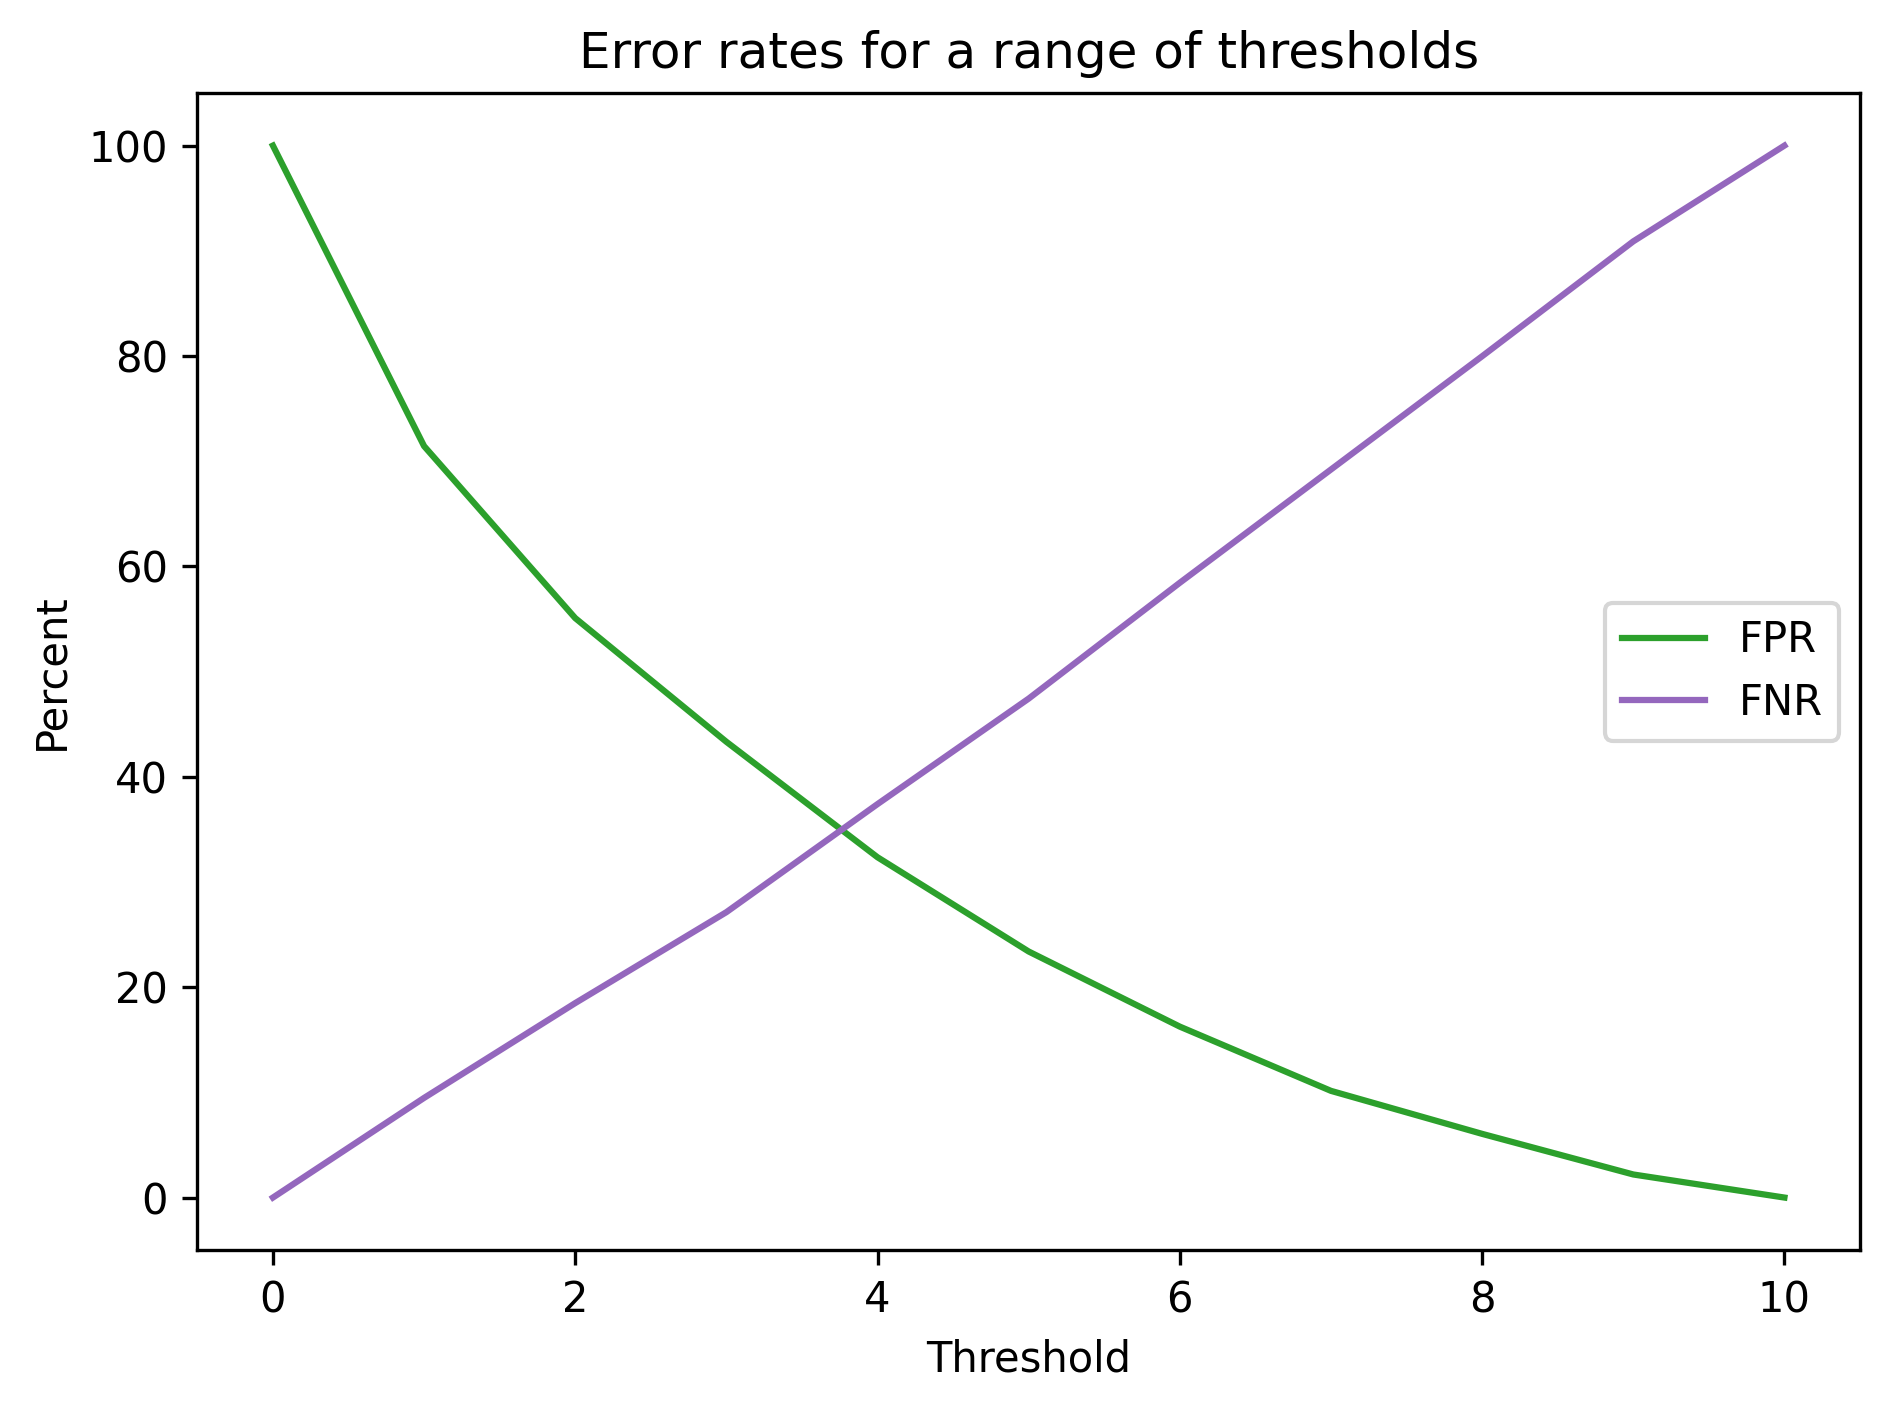
\includegraphics[width=4in]{chapters/02_calibration_files/02_calibration_36_0.png}
\end{center}

When the threshold is low, almost everyone is in the high risk group; in
that case:

\begin{itemize}
\item
  FNR is low because most recidivists are in the high risk group, but
\item
  FPR is high because most non-recidivists are \emph{also} in the high
  risk group.
\end{itemize}

When the threshold is high, almost everyone is in the low risk group,
and the metrics are the other way around:

\begin{itemize}
\item
  FPR is low because most non-recidivists are in the low risk group, but
\item
  FNR is high because most recidivists are \emph{also} in the low risk
  group.
\end{itemize}

The following figure shows predictive values for a range of thresholds.

\begin{lstlisting}[]
table_all['PPV'].plot(color='C0')
table_all['NPV'].plot(color='C1')

decorate(xlabel='Threshold', 
         ylabel='Percent',
         title='Predictive values for a range of thresholds')
\end{lstlisting}

\begin{center}
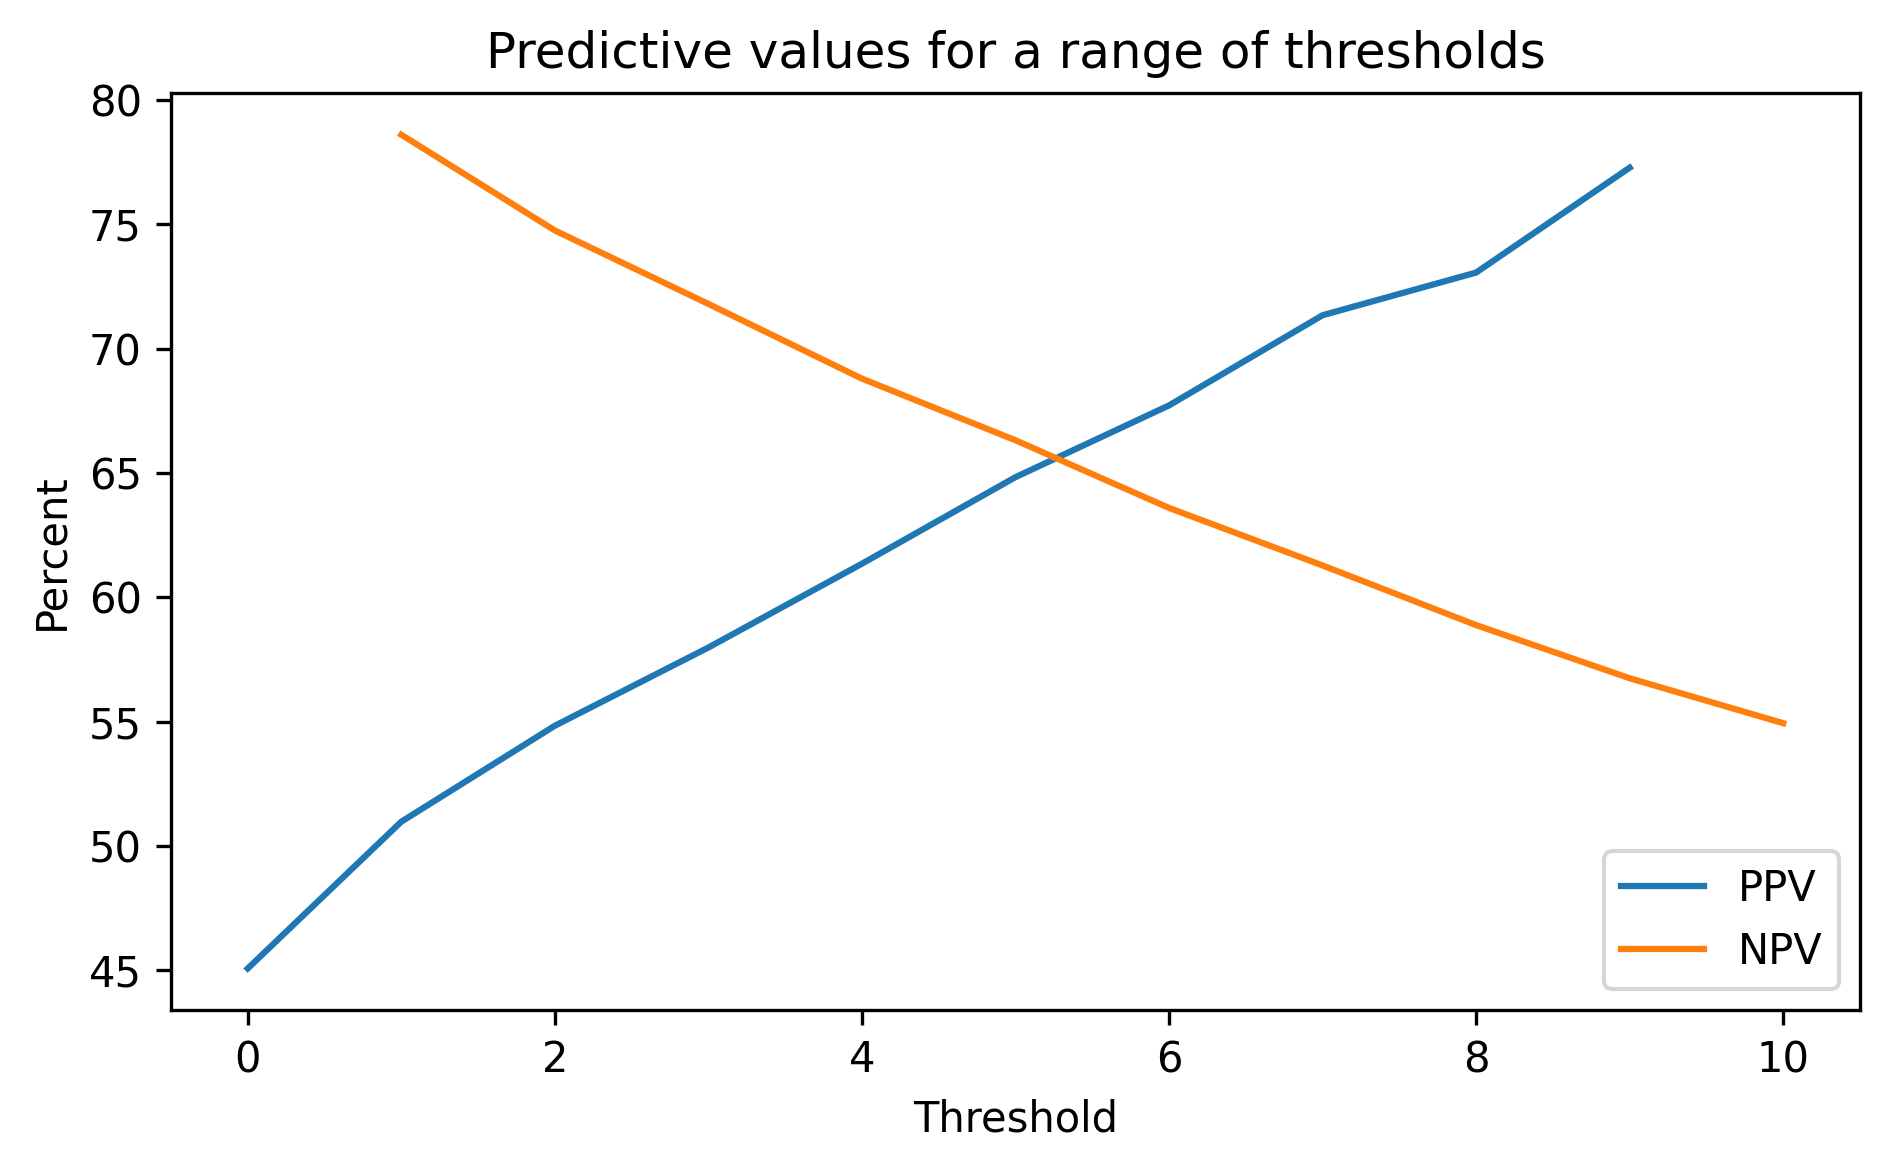
\includegraphics[width=4in]{chapters/02_calibration_files/02_calibration_38_0.png}
\end{center}

When the threshold is too low, PPV is low. When the threshold is too
high, NPV is low.

Now let's compute tables for Black and White defendants separately.

\begin{lstlisting}[]
table_white = sweep_threshold(cp[white])
table_black = sweep_threshold(cp[black])
\end{lstlisting}

We'll use the following function to interpolate columns in the table;
that is, for a given threshold I can compute the corresponding metric.

\begin{lstlisting}[]
from scipy.interpolate import interp1d

def interpolate(series, value, **options):
    """Evaluate a function at a value.
    
    series: Series
    value: number
    options: passed to interp1d (default is linear interp)
    
    returns: number
    """
    interp = interp1d(series.index, series.values, **options)
    return interp(value)
\end{lstlisting}

The following function goes the other way: it estimates the threshold
where a column passes through a given metric.

\begin{lstlisting}[]
def crossing(series, value, **options):
    """Find where a function crosses a value.
    
    series: Series
    value: number
    options: passed to interp1d (default is linear interp)
    
    returns: number
    """
    interp = interp1d(series.values, series.index, **options)
    return interp(value)
\end{lstlisting}

We can use \passthrough{\lstinline!crossing!} to calibrate the test for
White defendants; that is, we can compute the threshold that would make
the error rates for White defendants the same as for the general
population.

\begin{lstlisting}[]
matrix_all = make_matrix(cp)
fpr, fnr = error_rates(matrix_all)
\end{lstlisting}

\begin{lstlisting}[]
crossing(table_white['FPR'], fpr)
(@\dashfill@)
@@@array(3.23048519)@@@
\end{lstlisting}

\begin{lstlisting}[]
crossing(table_white['FNR'], fnr)
(@\dashfill@)
@@@array(3.11788885)@@@
\end{lstlisting}

With a threshold near 3.2, White defendants would have the same error
rates as the general population. Now let's do the same computation for
Black defendants.

\begin{lstlisting}[]
crossing(table_black['FPR'], fpr)
(@\dashfill@)
@@@array(5.20906103)@@@
\end{lstlisting}

\begin{lstlisting}[]
crossing(table_black['FNR'], fnr)
(@\dashfill@)
@@@array(5.01417524)@@@
\end{lstlisting}

To get the same error rates for Black and White defendants, we would
need different thresholds: about 5.1 compared to 3.2. At those levels,
the predictive values are substantially different. Here's PPV with
different thresholds for each group:

\begin{lstlisting}[]
interpolate(table_white['PPV'], 3.2)
(@\dashfill@)
@@@array(55.23319482)@@@
\end{lstlisting}

\begin{lstlisting}[]
interpolate(table_black['PPV'], 5.1)
(@\dashfill@)
@@@array(66.21639173)@@@
\end{lstlisting}

With equal error rates, we get different PPV:

\begin{itemize}
\item
  Among White defendants in the high risk group, about 55\% would
  recidivate.
\item
  Among Black defendants in the high risk group, about 66\% would
  recidivate.
\end{itemize}

Here's NPV with different thresholds for each group:

\begin{lstlisting}[]
interpolate(table_white['NPV'], 3.2)
(@\dashfill@)
@@@array(73.06639734)@@@
\end{lstlisting}

\begin{lstlisting}[]
interpolate(table_black['NPV'], 5.1)
(@\dashfill@)
@@@array(62.16782561)@@@
\end{lstlisting}

With equal error rates, the NPVs are substantially different:

\begin{itemize}
\item
  Among White defendants in the low risk group, 73\% went two years
  without another charge.
\item
  Among Black defendants in the low risk group, 62\% went two years
  without another charge.
\end{itemize}

To summarize, if the test is calibrated in terms of error rates, it is
not calibrated in terms of predictive values.

\begin{itemize}
\item
  If we make the error rates more equal, we make the predictive values
  more unfair, and
\item
  If we make the predictive values more equal, we make the error rates
  more unfair.
\end{itemize}

Fundamentally, the problem is that the prevalence of recidivism is
different in the two groups: about 39\% of White defendants were charged
with another crime within two years, compared to 51\% of Black
defendants. As long as that's the case (for any two groups) the
predictive values and error rates can't be ``fair'' at the same time.

That's the argument the Washington Post article presented. In the next
section, we'll take the argument one step farther by introducing one
more metric, the area under the ROC curve.

\hypertarget{roc-curve}{%
\section{ROC Curve}\label{roc-curve}}

In the previous section we plotted various metrics as as function of
threshold. Another common and useful way to visualize these results is
to plot sensitivity versus false positive rate (FPR). For historical
reasons, the result is called a \textbf{receiver operating
characteristic (ROC) curve}.

The following function plots the ROC curve:

\begin{lstlisting}[]
def plot_roc(table, **options):
    """Plot the ROC curve.
    
    table: DataFrame of metrics as a function of 
           classification threshold
    options: passed to plot
    """
    plt.plot([0,100], [0,100], ':', color='gray')
    sens = 100-table['FNR']
    plt.plot(table['FPR'], sens, **options)
    decorate(xlabel='FPR',
             ylabel='Sensitivity (1-FNR)',
             title='ROC curve')
\end{lstlisting}

Here's the ROC curve for all defendants.

\begin{lstlisting}[]
plot_roc(table_all, color='C2', label='All defendants')
\end{lstlisting}

\begin{center}
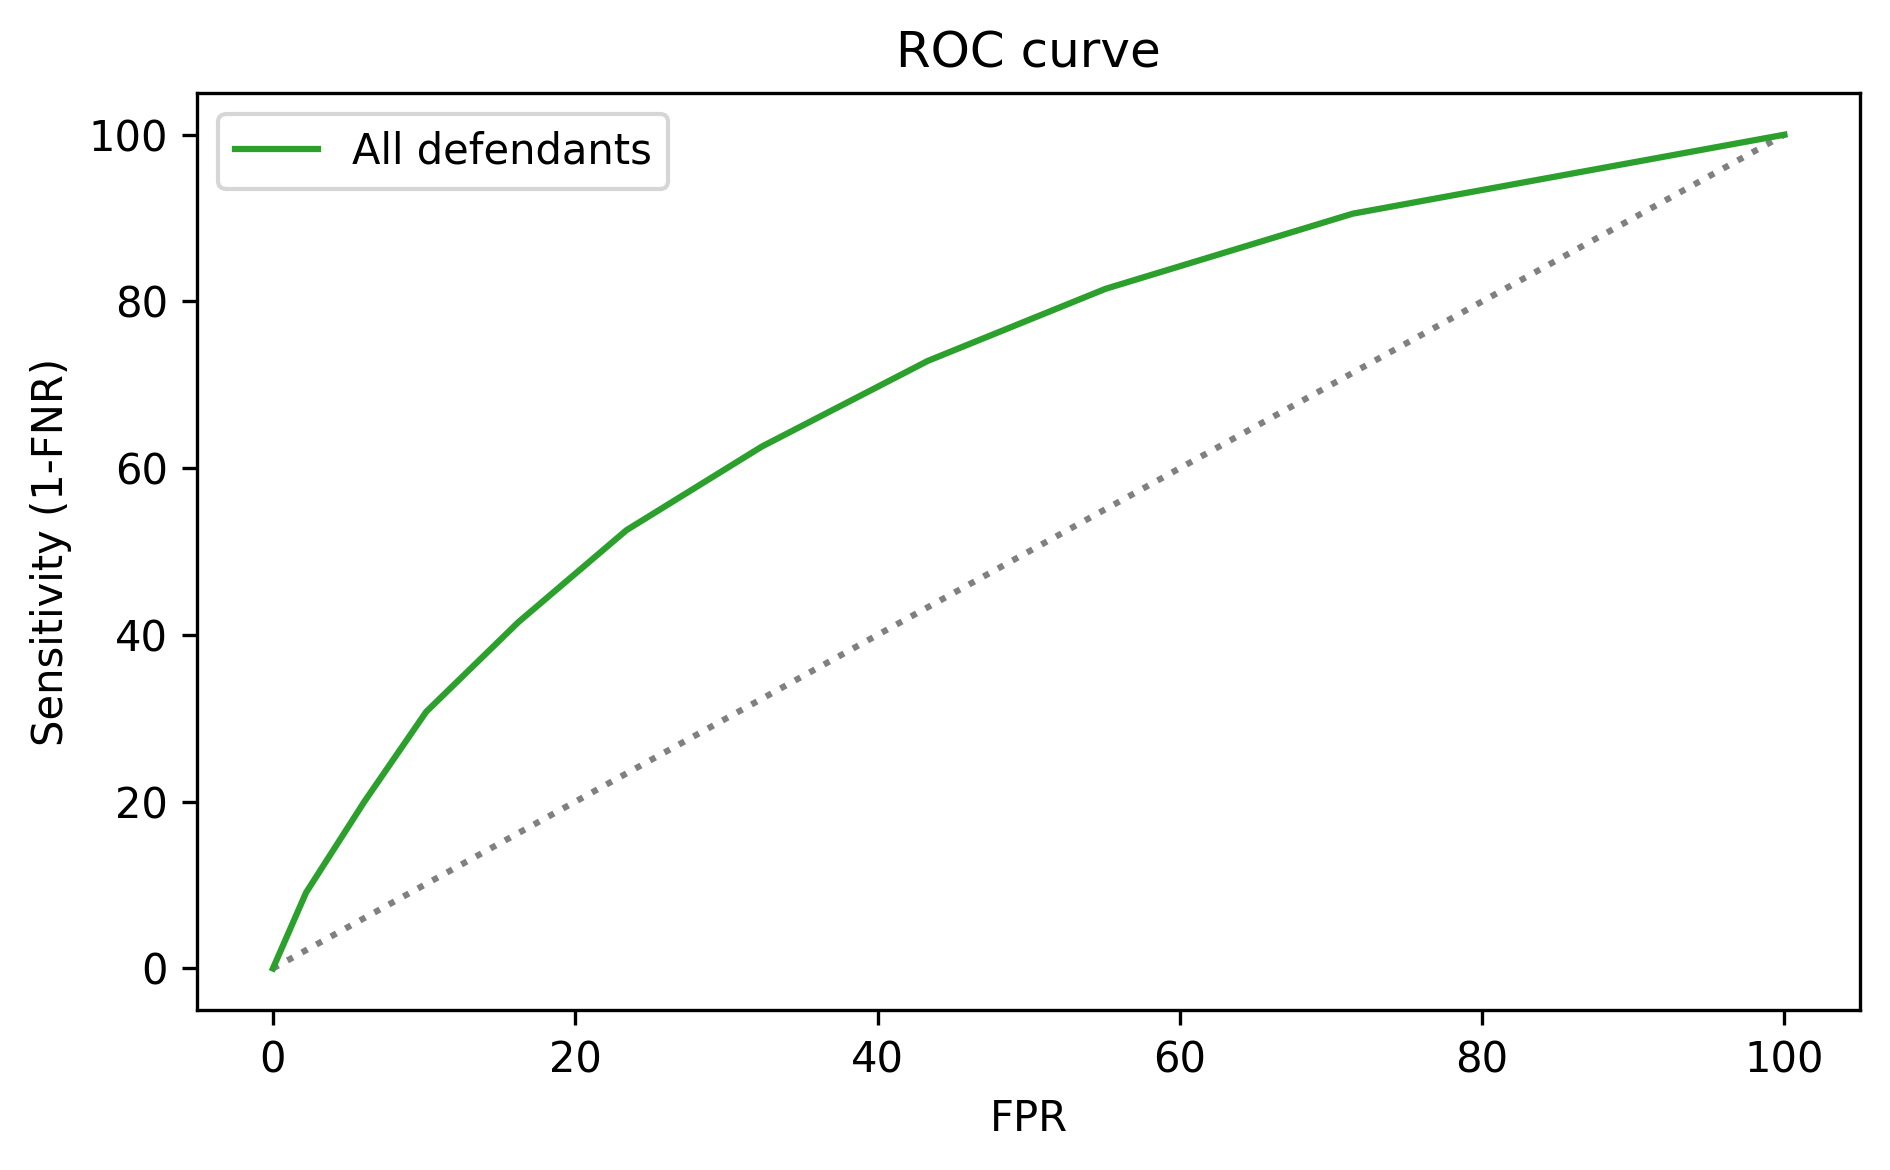
\includegraphics[width=4in]{chapters/02_calibration_files/02_calibration_63_0.png}
\end{center}

The green line is the ROC curve. The gray dotted line shows the identity
line for comparison.

An ideal test would have high sensitivity for all values of FPR, but in
reality there is almost always a trade-off:

\begin{itemize}
\item
  When FPR is low, sensitivity is low.
\item
  In order to get more sensitivity, we have to accept a higher FPR.
\end{itemize}

The ROC curve tells us how much sensitivity we get for a given FPR or,
the other way around, how much FPR we have to accept to achieve a given
sensitivity. The following figure shows the ROC curves for White and
Black defendants.

\begin{lstlisting}[]
plot_roc(table_white)
plot_roc(table_black)
\end{lstlisting}

\begin{center}
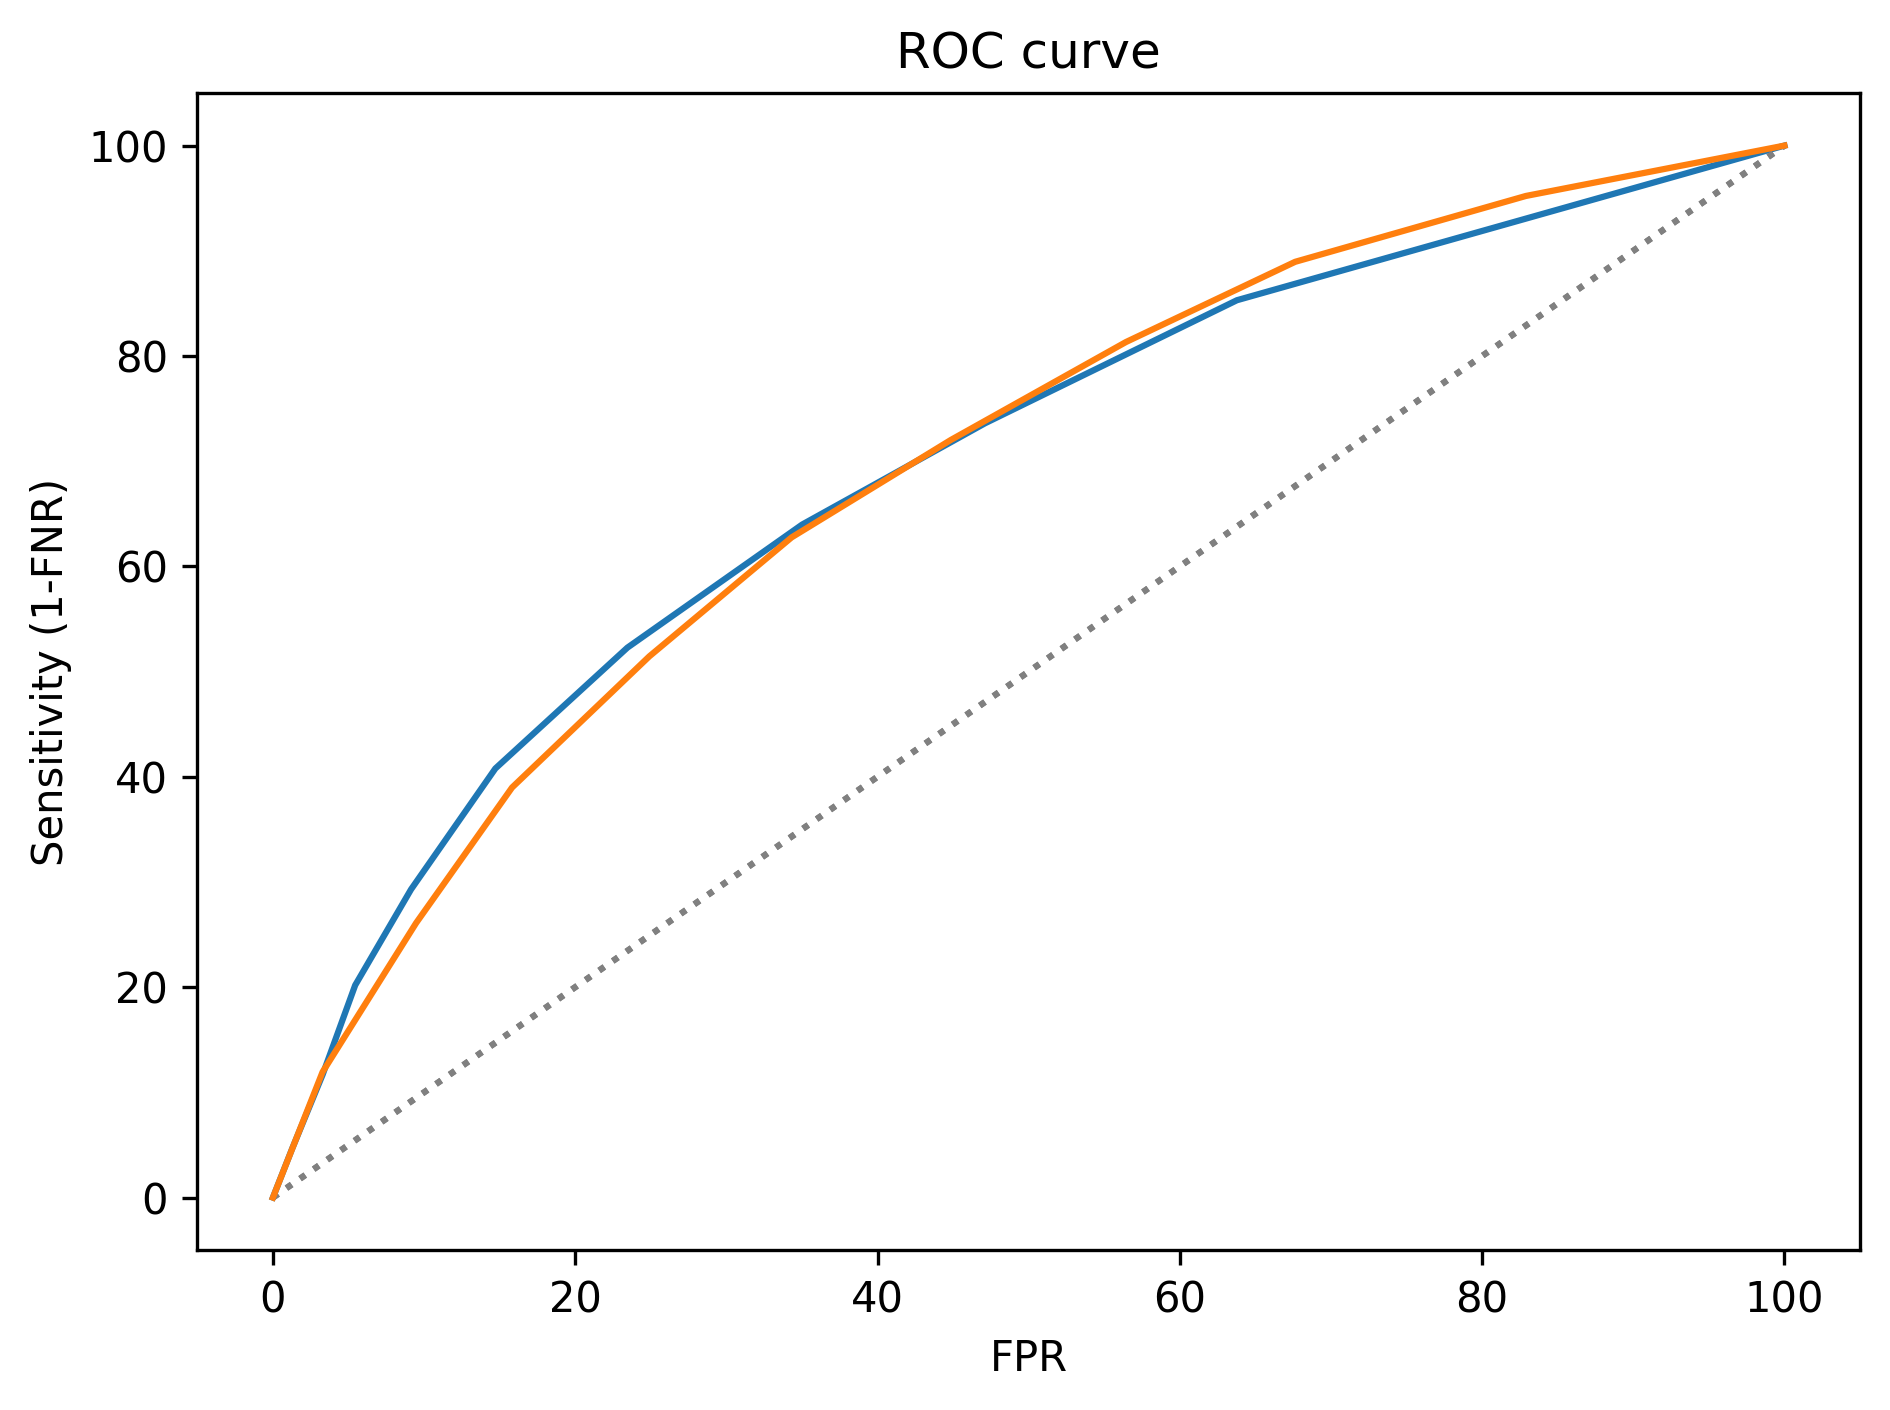
\includegraphics[width=4in]{chapters/02_calibration_files/02_calibration_65_0.png}
\end{center}

The ROC curves are similar for the two groups, which shows that we can
achieve nearly the same error rates (FPR and FNR) for the two groups, as
we did in the previous section. It also shows that the test has nearly
the same ``concordance'' for both groups, which I explain in the next
section.

\hypertarget{concordance}{%
\section{Concordance}\label{concordance}}

The authors of the ProPublica article published a supplementary article,
``How We Analyzed the COMPAS Recidivism Algorithm'', which describes
their analysis in more detail (see
\url{https://www.propublica.org/article/how-we-analyzed-the-compas-recidivism-algorithm}).

As another metric of accuracy, they estimate \textbf{concordance}, which
they describe like this:

\begin{quote}
Overall, {[}COMPAS has{]} a concordance score of 63.6 percent. That
means for any randomly selected pair of defendants in the sample, the
COMPAS system can accurately rank their recidivism risk 63.6 percent of
the time (e.g.~if one person of the pair recidivates, that pair will
count as a successful match if that person also had a higher score). In
its study, Northpointe reported a slightly higher concordance: 68
percent.
\end{quote}

They explain:

\begin{quote}
{[}These estimates{]} are lower than what Northpointe describes as a
threshold for reliability. ``A rule of thumb according to several recent
articles is that {[}concordances{]} of .70 or above typically indicate
satisfactory predictive accuracy, and measures between .60 and .70
suggest low to moderate predictive accuracy,'' the company says in its
study.
\end{quote}

There are several ways to compute concordance, but one of the simplest
is to compute the area under the ROC curve, which is why concordance is
also called the \textbf{area under the curve} or AUC. Since we've
already computed the ROC, we can use Simpson's rule to estimate the area
under the curve (see \url{https://en.wikipedia.org/wiki/Simpsons_rule}).

\begin{lstlisting}[]
from scipy.integrate import simps

def compute_auc(table):
    """Compute the area under the ROC curve."""
    y = 100-table['FNR']
    x = table['FPR']
    y = y.sort_index(ascending=False) / 100
    x = x.sort_index(ascending=False) / 100
    return simps(y.values, x.values)
\end{lstlisting}

The concordance for all respondents is about 70\%.

\begin{lstlisting}[]
compute_auc(table_all)
(@\dashfill@)
@@@0.7059974460900778@@@
\end{lstlisting}

For the subgroups it is slightly lower, but also near 70\%.

\begin{lstlisting}[]
compute_auc(table_white)
(@\dashfill@)
@@@0.6995093159638619@@@
\end{lstlisting}

\begin{lstlisting}[]
compute_auc(table_black)
(@\dashfill@)
@@@0.6945677570588521@@@
\end{lstlisting}

Different ways of computing concordance handle ties differently, which
is probably why we, ProPublica, and Northpointe get somewhat different
estimates. But qualitatively they all tell the same story; as a binary
classifier, COMPAS is only moderately accurate. However, it seems to be
equally accurate, by this metric, for White and Black defendants.

\hypertarget{summary}{%
\section{Summary}\label{summary}}

In this chapter, we replicated the analysis reported in the Washington
Post article and confirmed two of the arguments they presented:

\begin{enumerate}
\def\labelenumi{\arabic{enumi}.}
\item
  COMPAS is calibrated in the sense that White and Black defendants with
  the same risk score have almost the same probability of being charged
  with another crime. This implies that it has roughly the same
  predictive value for both groups.
\item
  It is impossible for COMPAS to have the same predictive values for
  both groups and the same error rates at the same time.
\end{enumerate}

And we showed:

\begin{itemize}
\item
  If you design a test to achieve equal predictive value across groups
  with different prevalence, you will find that error rates differ.
  Specifically, false positive rates will be higher in groups with
  higher recividism.
\item
  If you design a test to achieve equal error rates across groups, you
  will find that predictive values differ. Specifically, positive
  predictive value will be lower in groups with lower rates of
  recidivism.
\end{itemize}

Finally, we derived the ROC curve and computed AUC, which shows that
COMPAS has nearly the same concordance for White and Black defendants.

\hypertarget{discussion}{%
\section{Discussion}\label{discussion}}

If it is impossible to make a classification algorithm fair for all
groups, what should we do?

It might be tempting to forbid algorithms like COMPAS in the criminal
justice system, but unfortunately, that doesn't solve the problem. The
conclusions we reached in this case study apply to human decision-makers
as well, with the additional problem that humans are more unpredictable
than algorithms, and can be more biased. As long as we have to make
decisions about bail, sentencing, and parole, we will need data and
algorithms to inform those decisions, regardless of whether the
algorithms are run by humans or machines.

I don't have a solution to these problems, but I will suggest two
guidelines: the data we use should be unbiased, and the algorithms
should be transparent.

I discussed the problem of data bias in the previous chapter. In this
example, we used data about additional \emph{charges} as a measure of
additional \emph{crimes}. But not everyone who commits a crime gets
charged. If one group is more likely than another to be charged with a
crime, the algorithm will be unfair, no matter how it is calibrated.

Of course we should use unbiased data if we can, but if that's not
possible, sometimes we can do as well if we \emph{know} the data is
biased, in what directions, and by how much. So one thing we can do to
make algorithms more fair is to quantify biases in the data we use and
compensate for them.

Another thing we can do is make systems like COMPAS more transparent;
that is, we should know how they work, what factors they take into
account, and what they ignore. Algorithms intended to serve the public
interest should be the subject of public discussion, not the trade
secrets of a private company.

The use of algorithms in criminal justice, and in many other domains
that profoundly affect people's lives, is relatively new. It raises
difficult questions about fairness that we have only begun to recognize.

The goal of this case study is to help us measure the accuracy of these
algorithms and quantify their fairness. I hope it will contribute to the
ongoing debate as we address the many challenges of the criminal justice
system and the use of algorithms in our lives.

